SME Server es una distribución de Linux basada en CentOS. Está pensado para actuar como servidor en pequeñas y medianas empresas. Ofrece varios servicios, como alojamiento web, compartición de archivos e impresoras, Directorio Activo (LDAP), conexión a Internet y firewall, que podemos configurar muy fácilmente desde la interfaz web. Además, para una configuración más avanzada tenemos el sistema de Templates, del que hablaremos más adelante. Está mantenido por una comunidad de desarrolladores y su uso es gratuito incluso para organizaciones comerciales. Se financia solamente a base de donaciones.\\

Vamos a instalarlo en una máquina virtual. La primera pantalla que vemos nada más introducir el CD de instalación es la siguiente:

\begin{figure}[H]
    \centering
    \includegraphics[width=\textwidth]{capitulo02/00.png}
\end{figure}

Por defecto, el servidor usará los discos disponibles en modo RAID 1. Sin embargo podemos usar la segunda opción para elegir manualmente el nivel de RAID que queremos. Si seleccionamos 'Advanced installation options', nos llevará a un instalador gráfico en el que tendremos alguna opción más, como instalar el sistema en volúmenes de alacenamiento en la red, como iSCSI.

\begin{figure}[H]
    \centering
    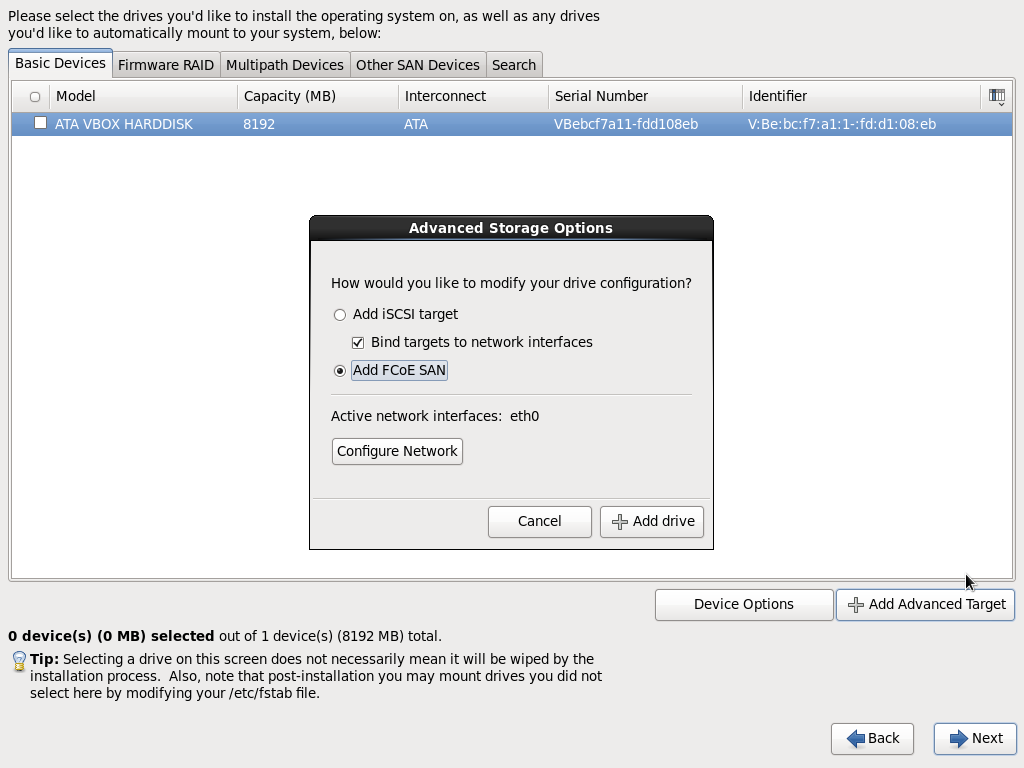
\includegraphics[width=\textwidth]{capitulo02/31instAv.png}
\end{figure}

La instalación borrará los discos completamente. No tenemos la opción de elegir el particionado manualmente. Por ejemplo, una máquina con 5 discos en RAID 5, este es el particionado que obtenemos tras la instalación:

\begin{figure}[H]
    \centering
    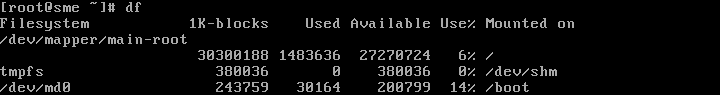
\includegraphics[width=\textwidth]{capitulo02/32raid5.png}
\end{figure}

En esta parte de la instalación solo podemos elegir el lenguaje y el tipo de teclado que vamos a utilizar. Cuando el sistema termina de instalarse, se reinicia y nos pregunta por varios aspectos de la configuración.

\section{Configuración inicial}

La primera vez que iniciamos la máquina tras instalar SME server tenemos que configurar el sistema. Nos pregunta por los siguientes parámetros:

\begin{itemize}
\item Contraseña del sistema.
\item Nombre del dominio y del sistema.
\item Configuración de la interfaz de red interna, asignación de IP y máscara.
\item Elegir el modo de operación del servidor.
\begin{figure}[H]
    \centering
    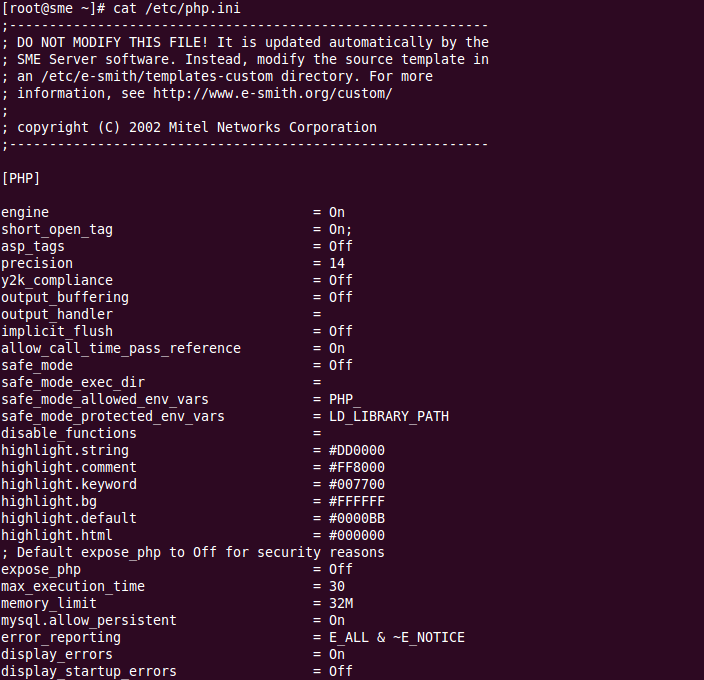
\includegraphics[width=\textwidth]{capitulo02/18.png}
\end{figure}
Tenemos 3 opciones:
\begin{itemize}
\item[\textbf{-}] \textbf{Server and gateway}. El servidor provee los servicios como email, web e intercambio de archivos e impresoras a la red interna y actúa como router y gateway entre la red interna e Internet. También actúa de firewall.
\item[\textbf{-}] \textbf{Private server and gateway}. Esta opción se diferencia del anterior en que los servicios que proporciona el servidor no son accesibles desde la red externa, y además el firewall contiene reglas adicionales.
\item[\textbf{-}] \textbf{Server-only mode}. En este modo, el servidor sólo se conecta a la red interna y ofrece los servicios ahí.
\end{itemize}
\item Configuración de la interfaz de red externa. Debemos decirle de qué manera se va a conectar a internet.
\begin{figure}[H]
  \centering
  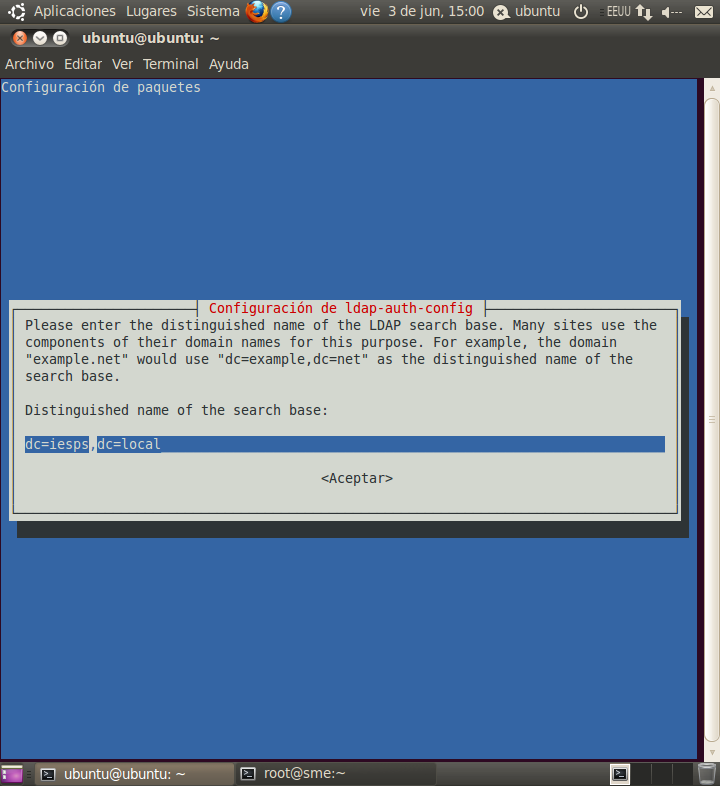
\includegraphics[width=\textwidth]{capitulo02/21.png}
\end{figure}
\item Configuración de un servicio de DNS dinámico.
\begin{figure}[H]
    \centering
    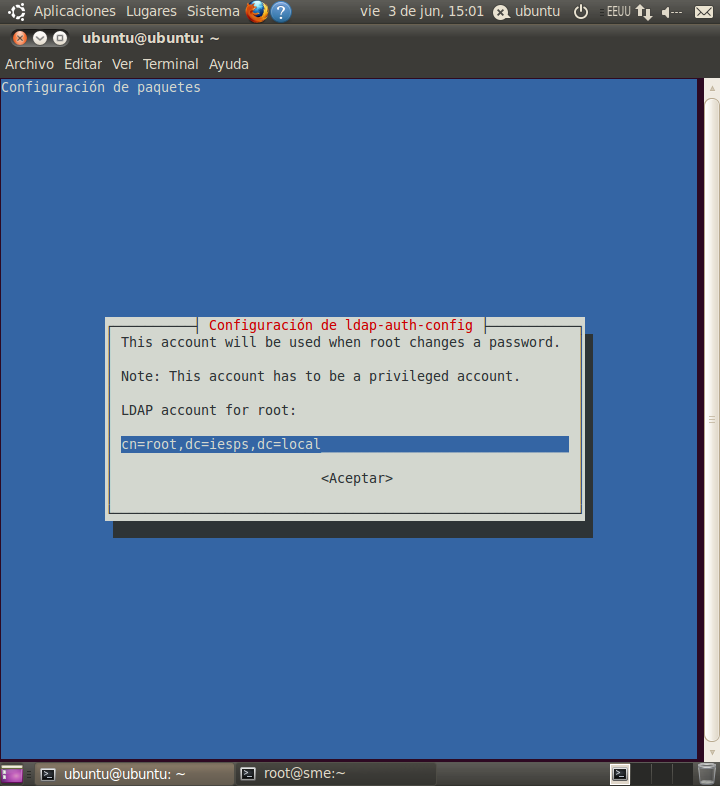
\includegraphics[width=\textwidth]{capitulo02/22.png}
\end{figure}
\item Configuración del DHCP para la red interna.
\item Por último nos pregunta si queremos usar otro servidor DNS que ya existiera en nuestra red interna.
\end{itemize}

En cuanto terminamos la configuración inicial ya tenemos un servidor completamente funcional ofreciendo distintos servicios. Vamos a ver sus características por defecto y las formas que tenemos de modificarlos.

\section{Modos de administración}

Existen varios modos distintos de adminstrar el SME server.

\subsection{Consola de root de Linux}

Al arrancar el sistema, accedemos con el usuario "root" y la contraseña de administración. Esto nos proporciona un acceso al sistema operativo mediante la terminal de Linux.\\

\begin{figure}[H]
    \centering
    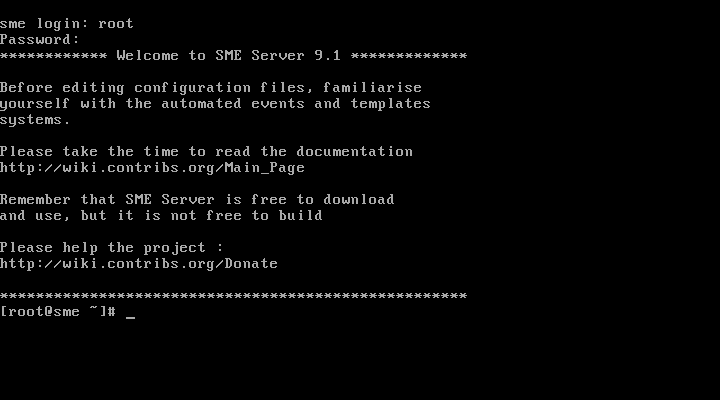
\includegraphics[width=\textwidth]{capitulo02/29.png}
\end{figure}

\subsection{Consola del servidor}

Al arrancar el sistema, accedemos con el usuario usuario "admin" y la contraseña de administración. También se puede acceder desde la consola de root, escribiendo "console".\\

\begin{figure}[H]
    \centering
    \includegraphics[width=\textwidth]{capitulo03/00.png}
\end{figure}

Tiene varias opciones
\begin{enumerate}
 \item \textbf{Check status of this server}: muestra el tiempo que ha estado en marcha el servidor.
\item \textbf{Configure this server}: nos lleva otra vez a través de las pantallas de la configuración inicial por si queremos cambiar algo.
\item \textbf{Test internet access}: prueba el acceso a internet mandando datos a contribs.org.
\item \textbf{Reboot, reconfigure or shut down this server}: reiniciar, reconfigurar o apagar el servidor.
\item \textbf{Manage disk redundancy}: muestra el estado de los discos y permite administrar el tipo de RAID. En nuestro caso solo hay un disco instalado... Parece que ha hecho 2 particiones (MIRAR).
\item \textbf{Access server manager}: permite acceder a la interfaz de administración web server-manager desde el mismo servidor usando el navegador en modo texto ELinks.
\item \textbf{View Support and licensing information}: ver la licencia (GNU GPL) e información sore cómo contactar con contribs.org para el soporte.
\item \textbf{Perform backup to removable media}: permite hacer un backup del estado actual del servidor en una unidad USB. La imagen se comprime en un archivo .tgz.
\item \textbf{Restore from removable media}: permite recuperar una imagen del servidor anteriormente guardada en una unidad USB.
\end{enumerate}

\subsection{Aceso remoto}
Podemos acceder a estos dos modos de administración desde otro PC a través de SSH, pero está desactivado por defecto:

\begin{figure}[H]
    \centering
    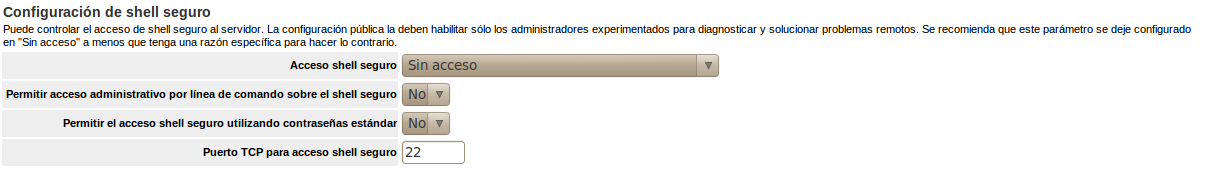
\includegraphics[width=\textwidth]{capitulo03/ssh00.png}
\end{figure}

En esta práctica permitiremos el acceso por SSH desde las redes locales para una administración más sencilla. Una vez activado, tendremos disponibles las dos primeras formas de administración que hemos explicado, dependiendo de si nos conectamos como 'root' o como 'admin'. SME server permite también el acceso mediante PPTP para la administración.

\subsection{Interfaz web server-manager}

SME Server provee una interfaz web de administración. Se accede desde el navegador de cualquier ordenador de la red interna con cualquiera de las siguientes URL:

\begin{itemize}
  \item https://sme/server-manager
  \item https://192.168.0.254/server-manager
\end{itemize}

\begin{figure}[H]
    \centering
    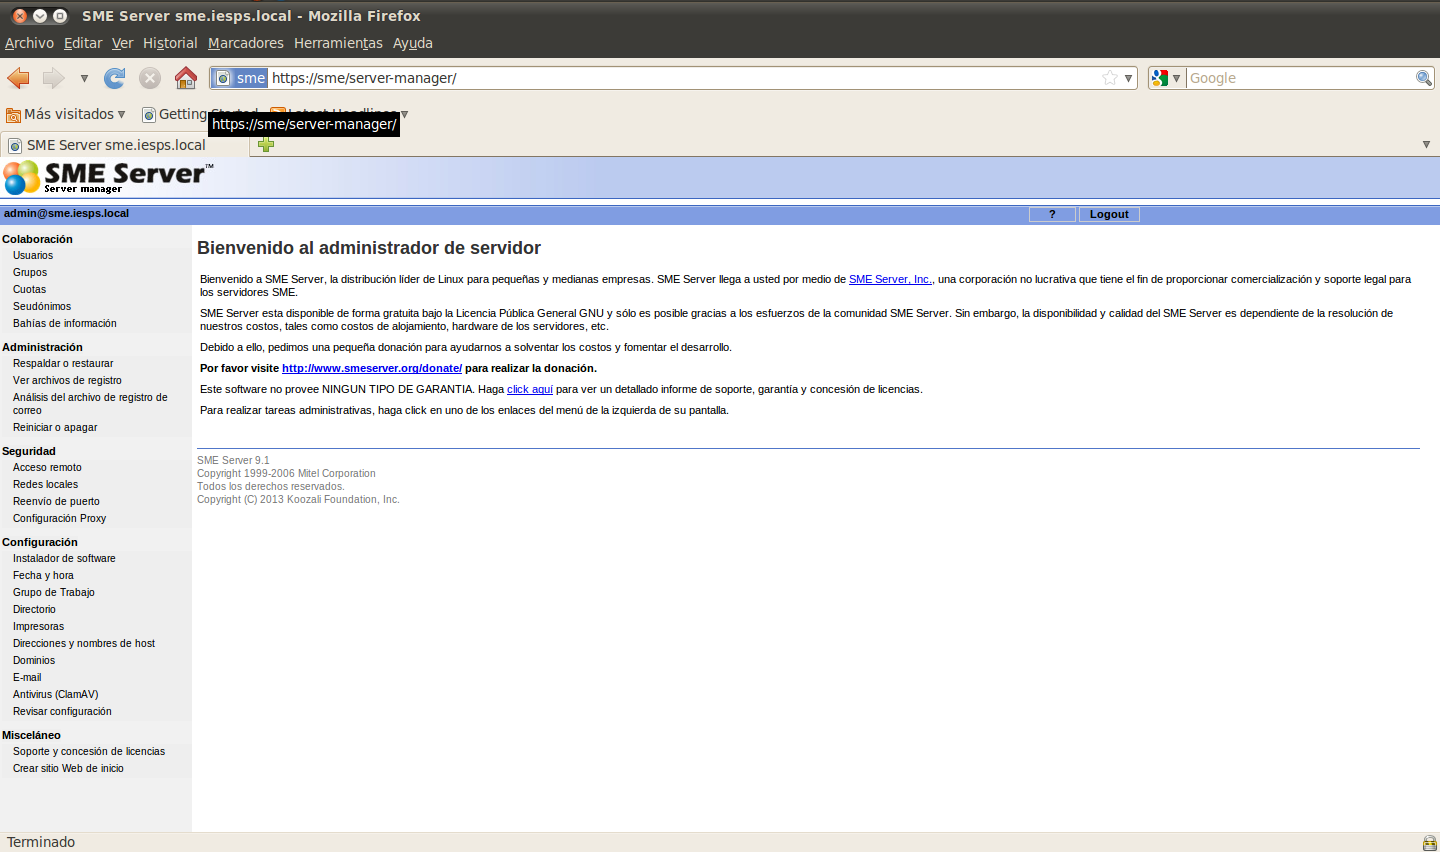
\includegraphics[width=\textwidth]{capitulo03/11.png}
\end{figure}

\section{Servicios y caracerísticas}

\begin{itemize}
\item Actúa como gateway, y proporciona un firewall, que luego veremos en más detalle. También actúa como servidor DNS.
\item Servidor Web.
\item Cuentas de usuario y grupos. Cada cuenta de usuario en SME server incluye una cuenta de email y un área de almacenamiento, en principio sin límite máximo, aunque se puede establecer.
\item Servidor de Directorio Activo.
\item Email. Existe la opción de reenviar los emails de un usuario o grupo a una cuenta externa. Se pueden crear varios pseudónimos para cada cuenta de email. SME nos da la opción de redirigir estos emails a una cuenta externa.
\item Almacenamiento. El área de almacenamiento de cada usuario está disponible con Samba. Aparte de esto, se pueden establecer bahías de información, o i-bays, que son directorios compartidos en el disco duro sobre los que podemos establecer fácilmente el control de acceso y los podemos proteger con contraseña.

\begin{figure}[H]
    \centering
    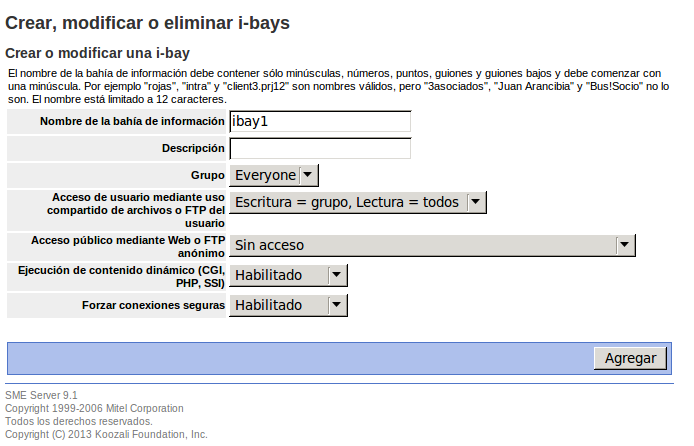
\includegraphics[width=\textwidth]{capitulo02/33.png}
\end{figure}

Los contenidos se encuentran en \lstinline!/home/e-smith/files/ibays/nombre_ibay/files!.
\end{itemize}
